\documentclass{article}
\usepackage{style}


\begin{document}

\begin{titlepage}
    \begin{center}
        \vspace*{1cm}

        \begin{figure}[H]
        \centering
        
\includegraphics[width=0.25\textwidth]{figures/logos/payload-designer.png}
        \end{figure}
    
        {\Huge\textbf{Payload Designer}}
            
        \bigskip
        \bigskip
        
        {\LARGE A design tool for the FINCH Eye payload}
            
        \bigskip
        \bigskip
        \bigskip
            
        {\Large Software Design Description \\}

        \vfill
        
        {\normalsize Designed and built by \\
        Payload Team \\
        Space Systems Division \\
        University of Toronto Aerospace Team \\}

        \bigskip
        \bigskip
        \bigskip
            
        {\Large \today}

        \begin{figure}[H]
            \centering
            
\includegraphics[trim={0 0 0 0}, clip, width=0.25\textwidth]{figures/logos/utat.png}
            % \caption{}
            \label{fig:logo} 
        \end{figure}
        
    \end{center}
\end{titlepage}







\begin{center}
    \texttt{
    David Maranto,
    Jennifer Zhang,
    Kejsi Gjerazi
    } \\
    University of Toronto
\end{center}


\tableofcontents
\newpage

\section{Introduction}
We present a \href{https://en.wikipedia.org/wiki/Software_design_description}{software design document} for the \textbf{payload designer} (hereafter referred to as the \texttt{program}): a high-level parametric design tool for the FINCH Eye hyperspectral imaging payload being developed by the University of Toronto Aerospace Team.

The objectives of the document are as follows:
\begin{itemize}
    \item Outline all parts of the software and how they will work in a cohesive system architecture.
    \item Address various design concerns and describe rationales for the adopted solutions.
    \item Act as a stable reference over the course of development.
    \item Coordinate the developer team under a single vision.
\end{itemize}

In other words, formally document all rough work including research, equations, references, and software design decisions. The development of such a tool is motivated by the payload team's need to arrive at refined component-specific requirements. As we have been finding through correspondence with component manufacturers, there are many component parameters that cannot be estimated from reference designs and rule-of-thumb estimates alone. Many are very much instrument-specific, and depend on the scientific objectives as well as many other coupled factors in the system. Attempts at modelling various aspects of the payload have been made (see the \href{http://spacesys.utat.ca/confluence/x/NoFmAQ}{Optics Toolkit}\footnote{Powered by Desmos, mankind's greatest invention. Second only to Python.}). These tools have sufficed for the first few design iterations of the payload (up to FINCH Eye v2) but have largely been disjoint and under-documented. Now that the payload team is entering the final stages of design, however, a more formal approach is warranted: one that enables a unified analysis of the entire payload and all of its components. This is the vision for the payload designer.

Source code for the project can be found on \href{https://github.com/spacesys-finch/payload-designer}{Github}.

\section{Design Values}
The following design values guide the design of the \texttt{program}.

\subsection{Modularity}
The adopted software system architecture strives to enable as much modularity and configurability as necessary to enable whatever types of analyses and tradeoff studies are desired. Component models are implemented using \href{https://en.wikipedia.org/wiki/Object-oriented_programming}{object-oriented programming} (OOP) to leverage the modularity of the paradigm. Similar components may inherit properties of a parent component (i.e. a VPH grating class may inherit methods and attributes from the surface-relief grating class). This reduces redundancy and the potential for buildup of technical debt.

\subsection{Usability}
The \texttt{program} strives to let the designer focus on the design as opposed to acting as a hindrance from it.  Configuration of design parameters is simple, allowing for rapid iteration, with little to no need to get into the gritty details of the implementation. The method used to construct new analyses is straightforward and intuitive. Outputs are reported in a user-friendly format, and leverage multi-dimensional visualization tools.

\subsection{Traceability}
The \texttt{program} and its supporting documentation strive to be traceable. This means all equations and mathematical derivations are traceable back to a \textit{source}, along with proper description of all assumptions associated with a particular model. This level of transparency is part of proper engineering practice as we mature the design of the payload.

\section{Functional Requirements}
Requirement language is to be interpreted as described in \href{https://microformats.org/wiki/rfc-2119}{RFC 2119}.

The \texttt{program} ...
\begin{enumerate}
    \item Must enable calculation of any quantity of interest associated with the payload given the parameters that define the quantity.
    \item Must allow for visualization of the parameter space for a given quantity to enable trade-off analyses.
    \item Should allow for automatic optimization of a quantity of interest given a parameter space and constraints.
    \item May expose controls and display results to a user-interface.
\end{enumerate}


\section{Scope \& Limitations} \label{sec:scope}
The following defines the scope of what the \texttt{program} intends to be and what it is not. A well-defined scope for the project is necessary to ensure the primary objectives of the project are met within the time constraints, and to avoid the development of functionality that may be redundant in the context of the other pre-existing tools available to the optics team.

\begin{itemize}
    \item \textbf{Closed-form equations}: All the equations that are used to model the payload system are closed-form. First- and/or second-order approximations are acceptable, such as the paraxial approximation. Consideration of higher-order phenomena such as \href{https://en.wikipedia.org/wiki/Optical_aberration}{optical aberrations} is better left to detailed simulations in CODE V\footnote{CODE V is the optic team's optical simulation tool.}
    \item \textbf{Ray tracing}: the \texttt{program} will \textbf{not} conduct \href{https://www.synopsys.com/glossary/what-is-ray-tracing.html}{ray tracing}. While a ray tracing engine would allow for the direct coupling of mechanical constraints with the system parameters, this is again better left to CODE V. The \texttt{program} is intended to be a high-level design tool. In effect, this limits the types of physical parameters that can be solved for to angles and relative distances.
\end{itemize}

\section{Platform}
The \texttt{program} is to be developed as a Python application. A number of development environments and platforms were considered. The rationale for converging on Python is traced below.

\begin{itemize}
    \item \textbf{Desmos:} High interactability with built-in sliders and plotting interface. High-fidelity visualization is possible, but requires considerable time investment to do right. Matrix algebra is possible, but requires some hacky solutions to implement. Quickly becomes cluttered and hard to document with more complex programs.
    
    \item \textbf{GeoGebra:} Big sister to Desmos. Matrix algebra is built-in, but same arguments of clutter and complexity apply as Desmos.
    
    \item \textbf{Google Colab:} Benefits of Python, plus sliders and other interactive UI elements easily creatable via markdown. Linear top-down structure may be limiting with respect to MathCAD.

    \item \textbf{GSOLVER:} Would produce the most accurate representation of our grating characteristics. Is only useful in the context of diffractor design, and may be excessive for our purposes. We should be alright with first- and second-order approximations of our diffractor models.
    
    \item \textbf{MathCAD:} Non-linear project structure makes for a more flexible development environment. Free version is very limited, and does not allow access to symbolic manipulation engine. Paid version is paid.
    
    \item \textbf{MATLAB:} Supports vectorization out of the box. MATLAB apps with a UI can be made fairly easily with sliders and plots, but the language is terrible. Period. MATLAB apps are nice, but can quickly become limiting compared to Python.
    
    \item \textbf{Python:} Greatest flexibility in most respects. \texttt{Numpy} allows for vectorized functions.  Can pair with \texttt{Tkinter} or \texttt{Pygame} to produce UI. Nice graphs are possible using \texttt{Plotly}. No support for function overloading. UI development is not as straightforward as a MATLAB app.
    
    \item \textbf{Unity:} Language supports function overloading. Would require team to learn C\#. Building the payload designer on top of an entire game engine may be excessive, and not at all lightweight to run and develop on.
\end{itemize}

\textit{\checkmark Recommendation: a Python application, with the potential for adding user-interactability through notebooks built using IPython in Google Colab.}

\section{System Architecture}

From a system architecture perspective, the payload designer can be seen as a collection of component models strung together in various arrangements or \textit{pipelines}. We describe component models and pipelines in turn.

\subsection{Components}
Component models are implemented as classes (see \href{https://docs.python.org/3/tutorial/classes.html}{Python documentation}), possessing attributes that define the parameters of the component, alongside methods that enable the calculation of attributes that are not initially defined.

\begin{figure}[H]
\centering
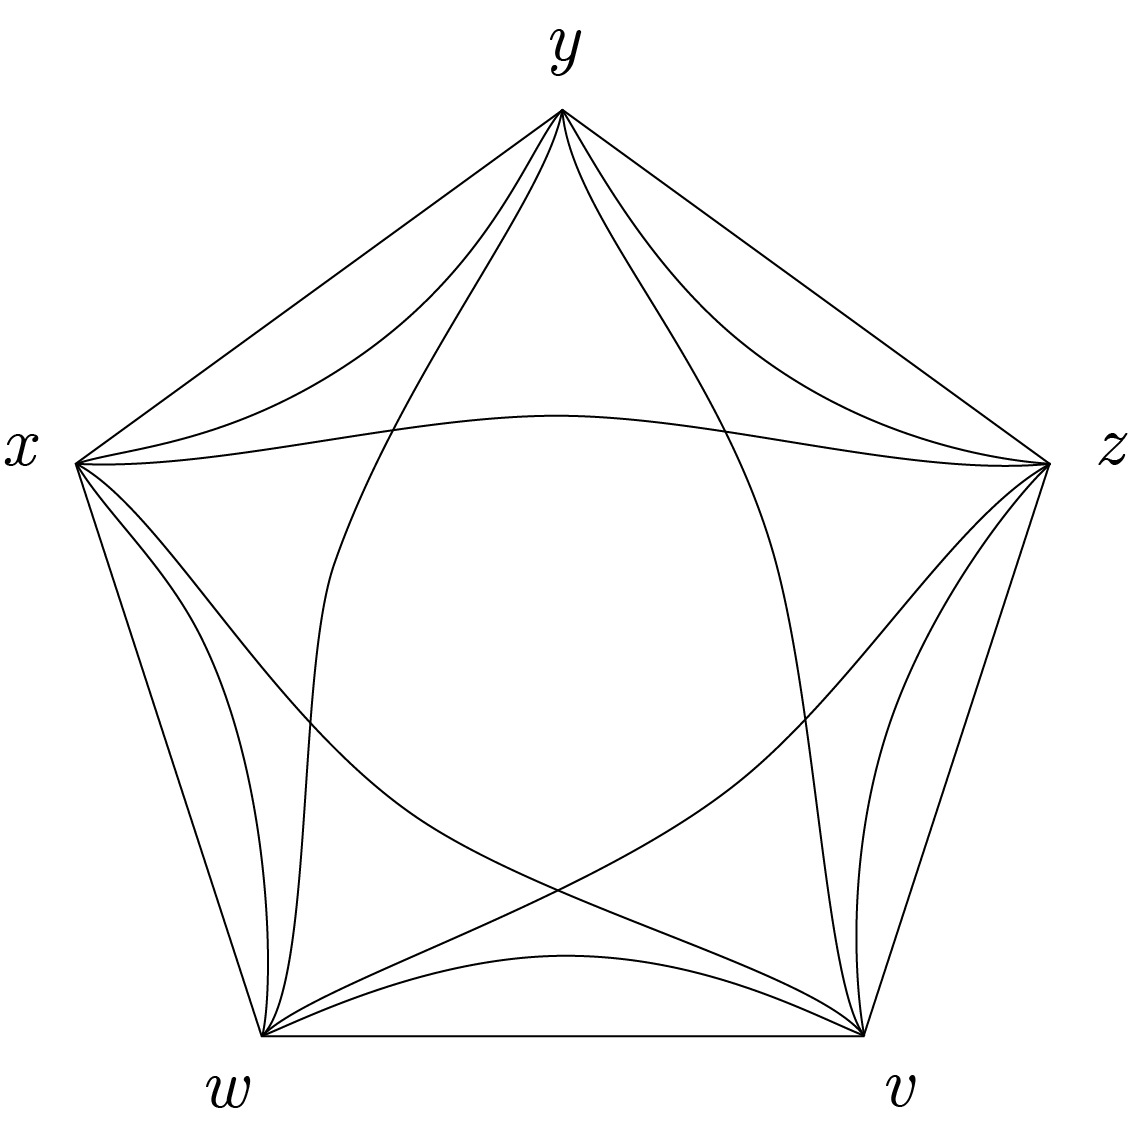
\includegraphics[width=0.5\textwidth]{figures/component-architecture.png}
\caption{Component class architecture.}
\label{fig:component-architecture}
\end{figure}

Where $v$, $w$, $x$, $y$, and $z$ are attributes defining the component. Connecting lines are methods used to compute an attribute given the other attributes it depends on. It should be noted that not every parameter is necessarily dependent on every other parameter which defines the component. The concept of input and output variables is dropped in favour of a general multi-directional dependency approach. This is done to provide the design team with as much flexibility as possible in their analysis. For example, a designer wishing to know the associated signal-to-noise ratio (SNR) for a particular slit width might build a pipeline that computes SNR as a function of slit width and all other required parameters. At a later time, the designer may wish to know the slit width required to reach a particular SNR target. To accomplish this, they would simply do some rewiring of the components in the pipeline. The internal logic of the component classes would adjust accordingly to compute slit width as a function of SNR.

\subsubsection{Vectorization}

\subsection{Pipelines}
A pipeline refers to a collection of components wired together to produce some output(s). 

\begin{figure}[H]
\centering
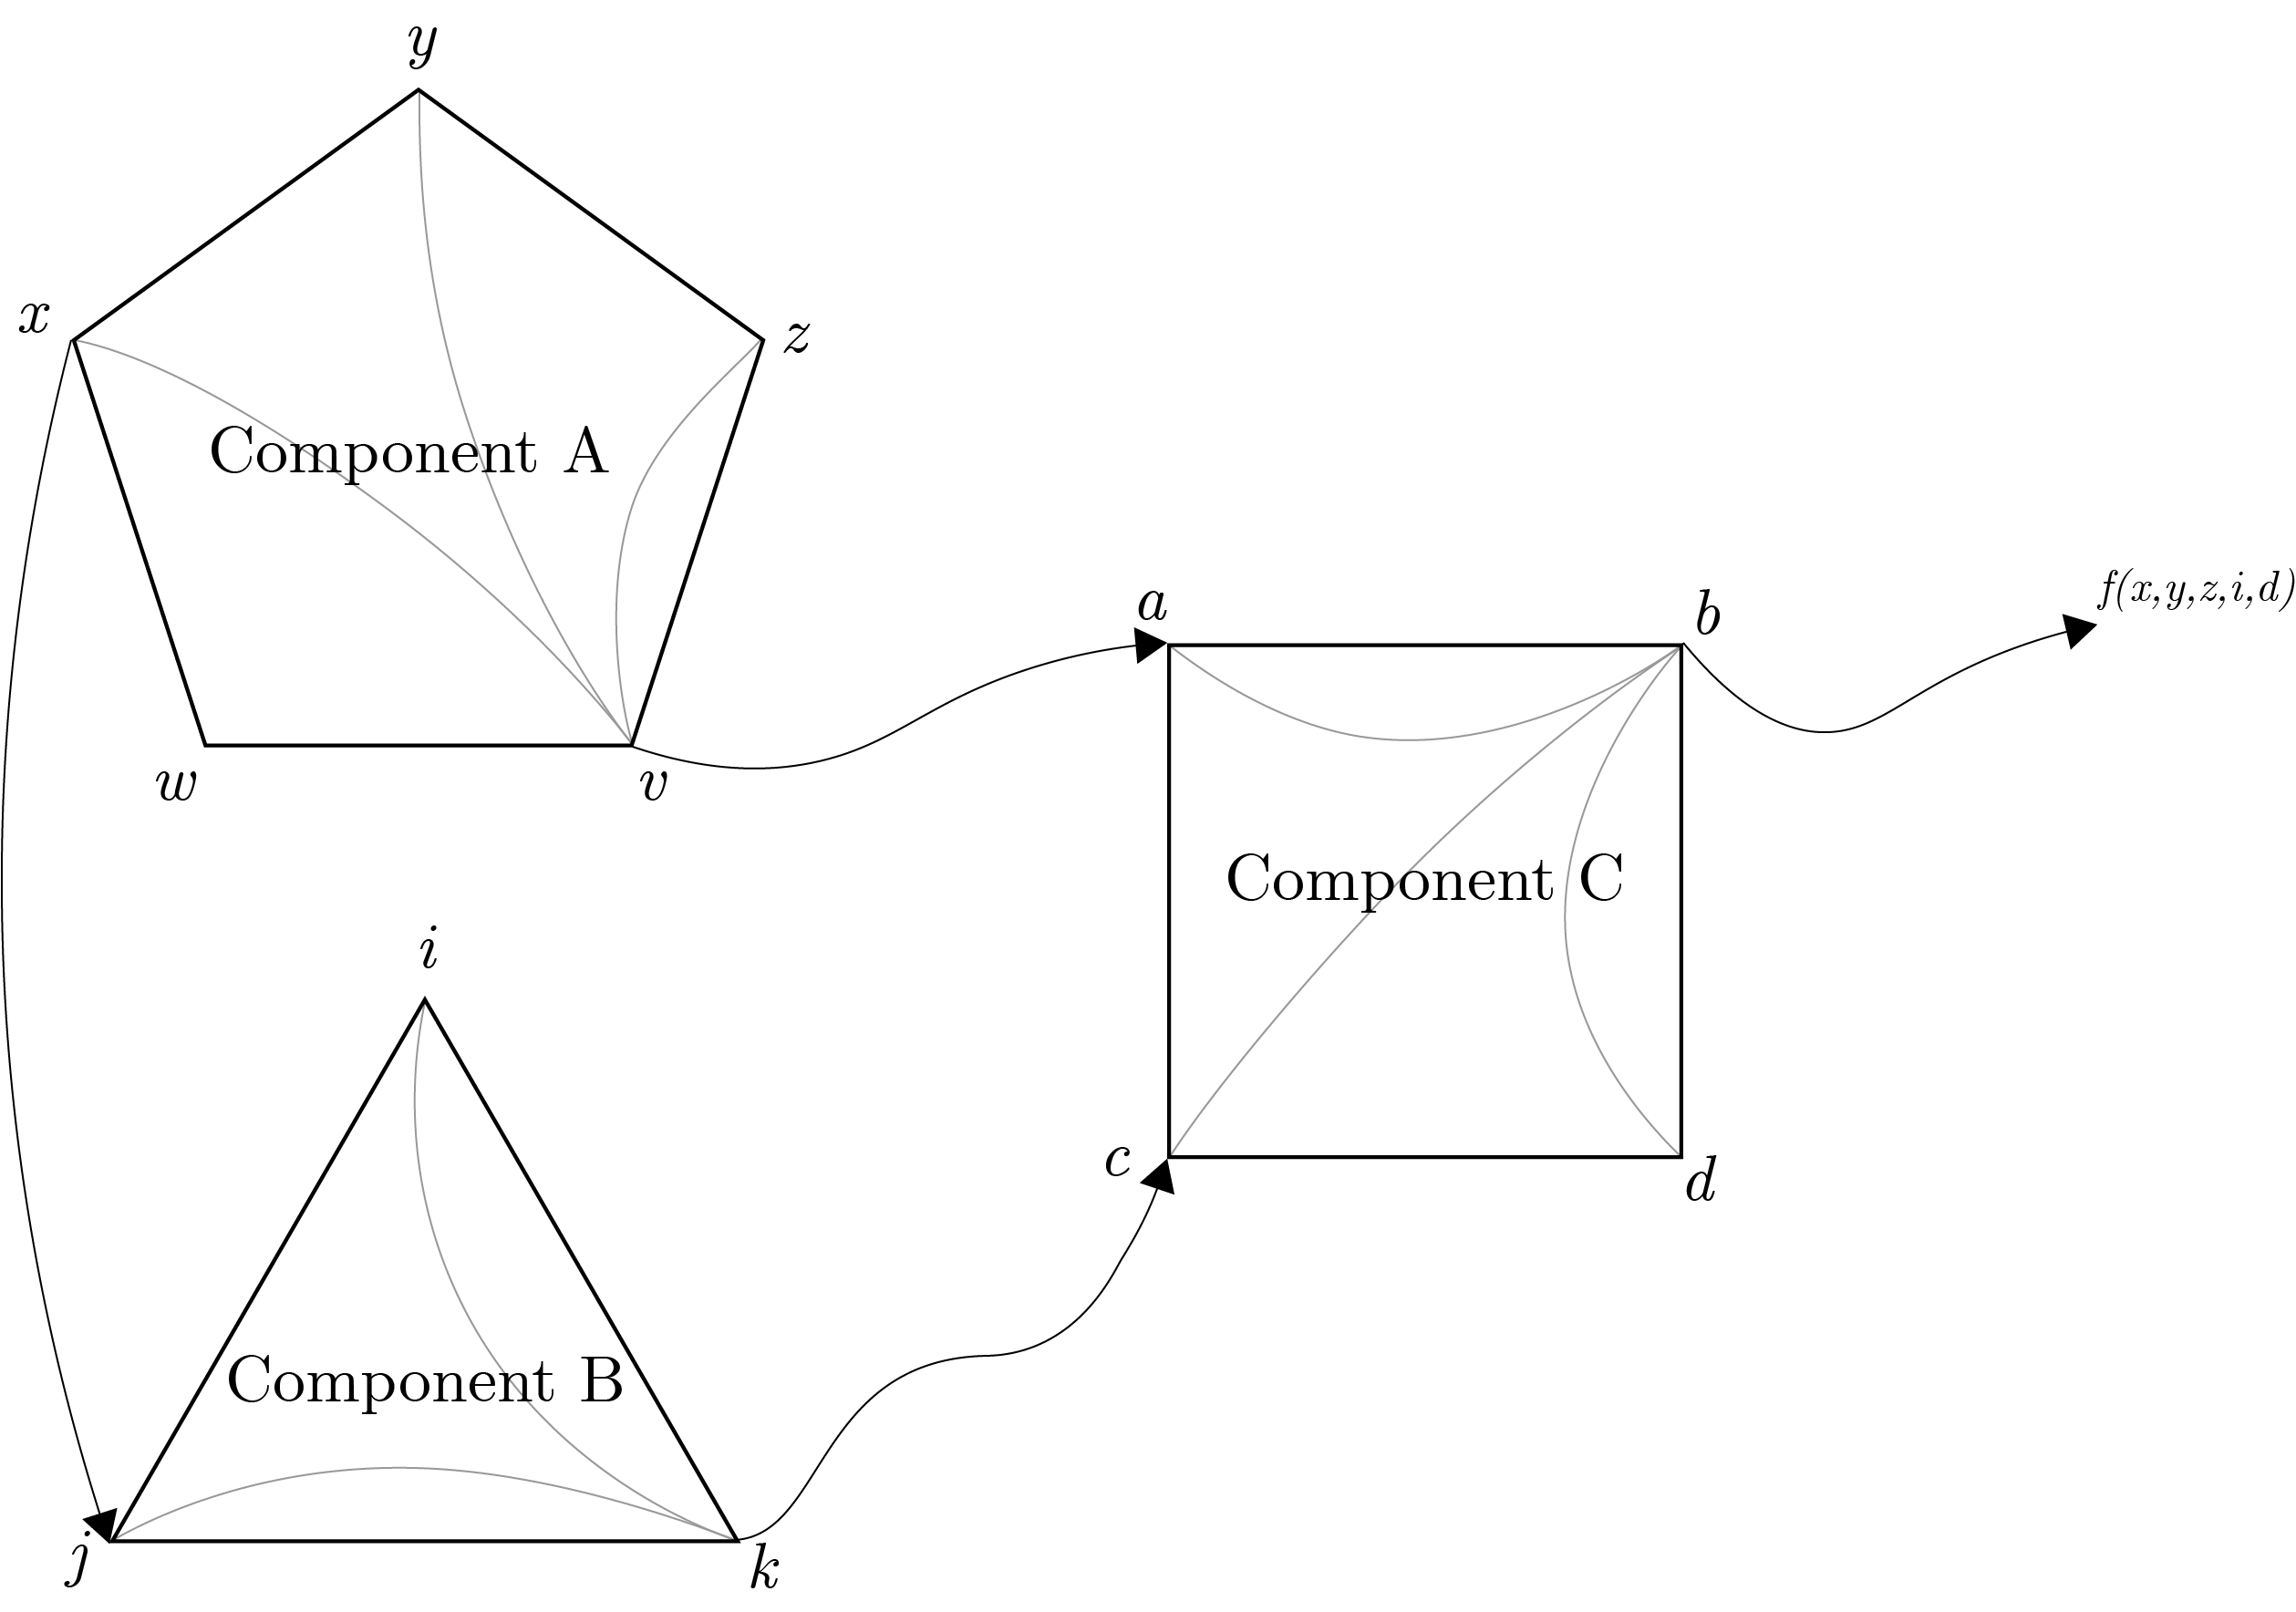
\includegraphics[width=0.75\textwidth]{figures/pipeline-architecture.png}
\caption{A generic pipeline architecture.}
\label{fig:pipeline-architecture}
\end{figure}

Practically, a pipeline is implemented in the following manner:

\begin{algorithm}
\caption{Component pipeline to solve for parameter $b$. A, B, and C are component classes.}\label{alg:pipeline}
\begin{algorithmic}

\Require $x, y, z, i, d$

\Comment{component instantiation}
\State $A.x \gets x$ 
\State $A.y \gets y$
\State $A.z \gets z$
\State $B.i \gets i$
\State $C.d \gets d$

\Comment{pipeline definition and propagation}
\State $j \gets A.x$
\State $a \gets A.v()$
\State $c \gets B.k(j)$

\State $b \gets C.b(a, c)$
\State \Return $b$

\end{algorithmic}
\end{algorithm}

\section{Project Stages}
The project is defined in four stages. These are:

\begin{itemize}
    \item \textbf{Stage 0}: Functional requirements are defined. Proposed system architecture is prototyped and validated. Developers are onboarded onto the payload designer development team and are familiarized with the toolchain.
    
    \item \textbf{Stage A}: Mathematical models for components are defined.
    
    \item \textbf{Stage B}: Components are implemented in source code. Visualization and optimization tools are implemented.
    
    \item \textbf{Stage C}: Numerical analysis and tradeoff studies begin. The component selection team defines component-specific requirements from findings. Parameters are validated and refined by the optical simulations team.
    
\end{itemize}

\section{Workflow}
The workflow for the development of component models (Stages A \& B) is described:

\begin{enumerate}
    \item A literature review is conducted on a specific component to source relevant parameters, equations, and typical values for the parameters that describe the component.
    \item A mathematical model created and presented in this document. Any required derivations are made and presented. The assumptions and limitations of the model are noted.
    \item Once the mathematical model for the component is peer-reviewed, it is implemented in the project source code.
    \item Unit tests are written to validate the functionality of the component class.
\end{enumerate}


\newpage
\printbibliography

\appendix
\appendixpage

\section{Derivations}



\subsection{Geometric Etendue}
Geometric etendue is calculated by \cite{Horiba_throughput_etendue}:

\begin{equation}
    d^2G = \frac{dS}{dQ}
\end{equation}

\begin{equation}
    G = \iint\frac{dS}{dQ}
\end{equation}

Where:
\begin{itemize}[label={}]
    \item $G$ [units]: Geometric etendue.
    \item $S$ [units]: Area of the emitting source.
    \item $Q$ [units]: Solid angle into which light propagates (2$\Omega$ in Figure \ref{fig:monochromator}).
\end{itemize}

Through integration:

\begin{equation}
    G = \pi\Sigma\sin^2\Omega
\end{equation}

Where:
\begin{itemize}[label={}]
    \item $G$ [units]: Geometric etendue.
    \item $\Omega$ [units]: Angle of the marginal ray from the optical axis.
\end{itemize}

\subsection{Source \& Image Distances}
\begin{enumerate}[(a)]
    \item In the case of a thin focuser, input rays are parallel, and may be represented by a source that is an infinite distance away. Output rays converge, hence the image is at a finite distance after the lens. Thus:
    \begin{equation}
        \frac{1}{f} = \lim_{d_o\to\infty} \frac{1}{d_o} + \frac{1}{d_i} = \frac{1}{d_i}
    \end{equation}
    
    \begin{equation} \label{eq:image-distance}
        \Rightarrow \ \boxed{d_i = f}    
    \end{equation}
    
    \item In the case of a thin collimator, incoming rays diverge, hence the source is at a finite distance before the lens. Outgoing rays are collimated, which may be represented by an image at an infinite distance away. Thus:
    \begin{equation}
        \frac{1}{f} = \lim_{d_i\to\infty} \frac{1}{d_o} + \frac{1}{d_i} = \frac{1}{d_o}
    \end{equation}
    
    \begin{equation} \label{eq:source-distance}
        \Rightarrow \ \boxed{d_o = f}
    \end{equation}
\end{enumerate}

\subsection{First-Order Model: Thin Lenses in Contact} - move to appendix
\todo{Note: these are Shiqi's derivations. Should be ok but would be good to find source.}

The simplest model assumes lenses are thin and in contact.

Definitions:
\begin{itemize}
    \item $f$: Equivalent focal length of the two lenses.
    \item $f_1$: Focal length of first (convex) lens. Positive.
    \item $f_2$: Focal length of second (concave) lens. Negative.
    \item $s_o$: Object distance of doublet. Equal to object distance of first lens.
    \item $s_i$: Image distance of doublet. Equal to image distance of second lens.
    \item $s_{i,1}$: Image distance of first lens. Equal to object distance of second lens.
\end{itemize}

For first (convex) lens:
\begin{equation}
    \frac{1}{f_1} = \frac{1}{s_o} + \frac{1}{s_{i,1}}
\end{equation}

For second (concave) lens:
\begin{equation}
    \frac{1}{f_2} = -\frac{1}{s_{i,1}} + \frac{1}{s_i}
\end{equation}

Together, by \eqref{eq:achromat-f_eq}:
\begin{align}
    \frac{1}{f} &= \frac{1}{f_1} + \frac{1}{f_2} \\
    &= \frac{1}{s_o} + \frac{1}{s_{i,1}} - \frac{1}{s_{i,1}} + \frac{1}{s_i} \\
    &= \frac{1}{s_o} + \frac{1}{s_i}
\end{align}

This is the Gaussian equation for the thin lens (as in \eqref{eq:thin-lens}), from which object and image distances as well as heights follow. We conclude that this simplified first-order model of an achromatic doublet is equivalent to a thin lens (achromatism is second-order). See Section \ref{sec:thin-singlet-model} for equations as well as their derivations for the focuser and collimator cases.

\textit{Note:} if we modelled the doublet as thin lenses with spacing $d$ between them, we would get the following equivalent focal length $f$ \cite{Boundless_undated-to}:
\begin{equation}
    \frac{1}{f} = \frac{1}{f_1} + \frac{1}{f_2} - \frac{d}{f_1 f_2}
\end{equation}
\textit{}

\section{Constants}
Table \ref{tab:constants} lists the exact values for the scientific constants used in calculations.

\begin{table}[H]
\centering
\caption{Table of constants. Taken from the \href{https://docs.astropy.org/en/stable/constants/index.html}{Astropy} Python package.}
\label{tab:constants}
\begin{tabular}{@{}llll@{}}
\toprule
Constant               & Symbol  & Value                        & Unit                             \\ \midrule
Gravitational Constant & {$G$}   & {\num{6.6743e-11}}           & {\si{\m\cubed\per\kg\s\squared}} \\
Mass of Earth          & {$M_E$} & {\num{5.972167867791379e24}} & {\si{\kg}}                       \\
Planck's Constant      & {$h$}   & {\num{6.62607015e-34}}       & {\si{\joule\s}}                  \\
Radius of Earth        & {$R_E$} & {\num{6378.1}}               & {\si{\km}}                       \\
Speed of Light         & {$c$}   & {\num{299792458}}            & {\si{\m\per\second}}             \\ \bottomrule
\end{tabular}
\end{table}

\subsection{Resolvance} \label{sec:resolvance}
Diffraction gratings have multiple grooves that follow the same relations as a double slit. The expression for resolving power of a grating is derived by using the intensity expression for a double slit grating. 

\begin{figure}[H]
\centering
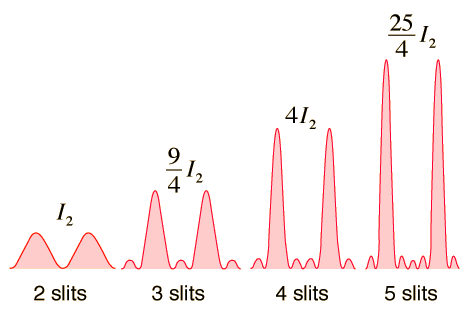
\includegraphics[width=0.5\textwidth]{figures/grating_intensity_curves.png}
\caption{The intensity curves for gratings with varying numbers of slits. Increasing the slits improves the resolution by sharpening the intensity curves.}
\label{fig:grating-intensity}
\end{figure}

The peaks have a phase difference of $\delta$ = 2m$\pi$. The closest minimums occur $\frac{\pi}{2}$ away from the peak, which occurs for a phase change of: 
\begin{equation}
\Delta \delta = \frac{2\pi}{N}
\end{equation}
Where N is the number of slits.

\begin{figure}[H]
\centering
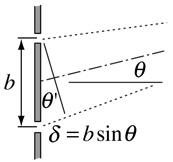
\includegraphics[width=0.5\textwidth]{figures/grating-set-up.png}
\caption{A two-slit grating showing the parameters b, $\theta$, and $\delta$}
\label{fig:grating-set-up}
\end{figure}

From the figure, 
\begin{equation}
\delta = \frac{2\pi}{\lambda}b\sin{\theta}
\end{equation}
The differential of the above is: 
\begin{equation}
d\delta = \frac{2\pi}{\lambda}b\cos{\theta}d\theta
\end{equation}
The maximum condition is:
\begin{equation}
b\sin{\theta} = m\lambda
\end{equation}
With the differential:
\begin{equation}
b\cos{\theta}d\theta = md\lambda
\end{equation}
Substituting both differentials gives:
\begin{equation}
\frac{2\pi}{N} = \frac{2\pi}{\lambda}md\lambda
\end{equation}
This simplifies to the final resolving power formula \cite{Hyperphysics}:
\begin{equation}
\boxed{R = \frac{\lambda}{\Delta \lambda} = mN}
\end{equation}

Where:
\begin{itemize}[label={}]
    \item $\lambda$ is the wavelength of interest.
    \item $\Delta \lambda$ is the resolution.
    \item $m$ is the diffraction order
\end{itemize}

\include{nomenclature}


\end{document}
